\documentclass{beamer}

\usepackage{graphicx}
\usepackage{tikz}

\setbeamertemplate{navigation symbols}{}%remove navigation symbols

\title{The Mathematics of Rock Paper Scissors}
\author{Vince Knight}
\date{23/05/2013}

\begin{document}

\frame{
\begin{center}
\includegraphics[width=\textwidth]{purity.png}
\end{center}
}

\frame{
\huge
\begin{center}
\begin{tabular}{|c|c|c|c|c|}
\hline
0& -1& 1& 1& -1\\
\hline
1& 0& -1& -1& 1\\
\hline
-1& 1& 0& 1 & -1\\
\hline
-1& 1& -1& 0& 1\\
\hline
1& -1& 1& -1& 0\\
\hline
\end{tabular}
\end{center}
}

\frame{
\begin{center}
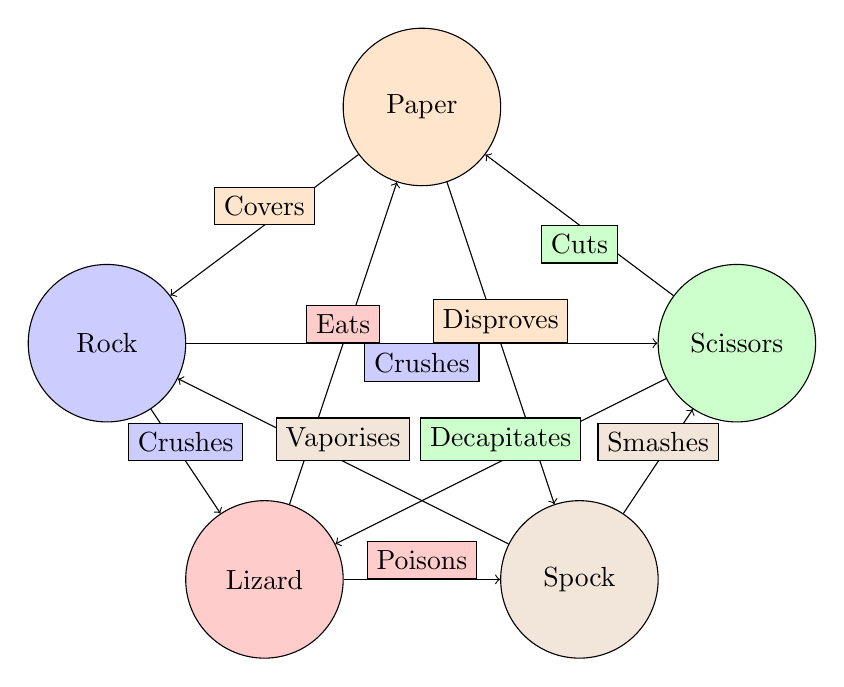
\begin{tikzpicture}

\node (R) at (0,0) [circle, minimum width = 2cm, draw, fill=blue!20] {Rock};
\node (P) at (4,3) [circle, minimum width = 2cm, draw, fill=orange!20] {Paper};
\node (S) at (8,0) [circle, minimum width = 2cm, draw, fill=green!20] {Scissors};
\node (Lz) at (2,-3) [circle, minimum width = 2cm, draw, fill=red!20] {Lizard};
\node (Sp) at (6,-3) [circle, minimum width = 2cm, draw, fill=brown!20] {Spock};

\draw [->] (P) -- node[above, fill=orange!20, draw] {Covers} (R);
\draw [->] (P) -- node[above, fill=orange!20, draw] {Disproves} (Sp);

\draw [->] (R) -- node[below, fill=blue!20, draw] {Crushes} (S);
\draw [->] (R) -- node[above, fill=blue!20, draw] {Crushes} (Lz);

\draw [->] (S) -- node[below, fill=green!20, draw] {Cuts} (P);
\draw [->] (S) -- node[above, fill=green!20, draw] {Decapitates} (Lz);

\draw [->] (Lz) -- node[above, fill=red!20, draw] {Eats} (P);
\draw [->] (Lz) -- node[above, fill=red!20, draw] {Poisons} (Sp);

\draw [->] (Sp) -- node[above, fill=brown!20, draw] {Vaporises} (R);
\draw [->] (Sp) -- node[above, fill=brown!20, draw] {Smashes} (S);
\end{tikzpicture}
\end{center}
}

\frame{
``I play Rock 20\% of the time and Spock the rest of the time."
{\huge
\begin{center}
\begin{tabular}{|c|c|c|c|c|}
\hline
\textbf{0}& -1& 1& 1& \textbf{-1}\\
\hline
\textbf{1}& 0& -1& -1& \textbf{1}\\
\hline
\textbf{-1}& 1& 0& 1 & \textbf{-1}\\
\hline
\textbf{-1}& 1& -1& 0& \textbf{1}\\
\hline
\textbf{1}& -1& 1& -1& \textbf{0}\\
\hline
\end{tabular}
\end{center}}
\pause
$$
u(R) = 0.2\times0+0.8\times(-1)=-0.8
$$
}

\frame{
\begin{align*}
u(R) &= 0.2\times0+0.8\times(-1)=-0.8\\
u(P) &= 0.2\times1+0.8\times(1)=1\\
u(S) &= 0.2\times(-1)+0.8\times(-1)=-1\\
u(Lz) &= 0.2\times(-1)+0.8\times(1)=0.6\\
u(Sp) &= 0.2\times1+0.8\times(0)=0.2\\
\end{align*}
}

\frame{
\includegraphics[width=\textwidth]{plot.pdf}
}

\frame{
\begin{itemize}
    \item Economics: how companies trade;
    \item Computer Science: how servers interact;
    \item Biology: evolution.
\end{itemize}
}

\frame{
\begin{center}
{\huge{Mathematics}}
\end{center}
}

\end{document}
